\documentclass{beamer}

\usepackage[czech]{babel}
\usepackage[utf8]{inputenc}
\usepackage[T1]{fontenc}
\usepackage{lmodern}
\usepackage{datetime}
\usepackage{tikz}
\usepackage{amssymb}
\usepackage{bbding}
\usepackage{tabularx}

\usetikzlibrary{shadows}
% Themes: http://www.hartwork.org/beamer-theme-matrix/
\mode<presentation>{\usetheme{Madrid}}
\usecolortheme{beaver}
\beamertemplatenavigationsymbolsempty
\setbeamertemplate{title page}[default][colsep=0bp,rounded=true]
\setbeamertemplate{itemize items}{$\star$}
\setbeamercolor*{item}{fg=black}
\setbeamertemplate{enumerate item}[default]
\newcommand{\Has}{\textcolor{green}{\CheckmarkBold}}
\newcommand{\NoHas}{\textcolor{red}{\XSolidBrush}}

\newenvironment<>{positiveblock}[1]{%
  \begin{actionenv}#2%
      \def\insertblocktitle{#1}%
      \par%
      \mode<presentation>{%
        \setbeamercolor{block title}{fg=white,bg=green!20!black}
       \setbeamercolor{block body}{fg=black,bg=green!50}
       \setbeamercolor{itemize item}{fg=green!20!black}
       \setbeamertemplate{itemize item}[triangle]
     }%
      \usebeamertemplate{block begin}}
    {\par\usebeamertemplate{block end}\end{actionenv}}
    
\newenvironment<>{negativeblock}[1]{%
  \begin{actionenv}#2%
      \def\insertblocktitle{#1}%
      \par%
      \mode<presentation>{%
        \setbeamercolor{block title}{fg=white,bg=red!20!black}
       \setbeamercolor{block body}{fg=black,bg=red!35}
       \setbeamercolor{itemize item}{fg=red!20!black}
       \setbeamertemplate{itemize item}[triangle]
     }%
      \usebeamertemplate{block begin}}
    {\par\usebeamertemplate{block end}\end{actionenv}}


\author{Vojtěch Boček}
%\institute[vbocek@gmail.com]{SPŠ a VOŠ technická, Sokolská 1, Brno \\[0.5cm] \includegraphics[width=2cm]{logo-skoly}}
\institute[vbocek@gmail.com]{SPŠ a VOŠ technická Brno, Sokolská 1\\[0.5cm]}
\title{LORRIS TOOLBOX}
\subtitle{Sada nástrojů pro vývoj a~řízení robotů}
\date[]{}

%\newdate{date}{13}{03}{2013}
%\date{\displaydate{date}}


\begin{document}


\frame{\titlepage}

\begin{frame}
    \frametitle{Vývoj techniky -- mechanika}
    \begin{center}
	    \begin{tikzpicture}
		  \node[drop shadow={shadow xshift=.8ex,shadow yshift=-.8ex},fill=white,draw] at (0,0) {   		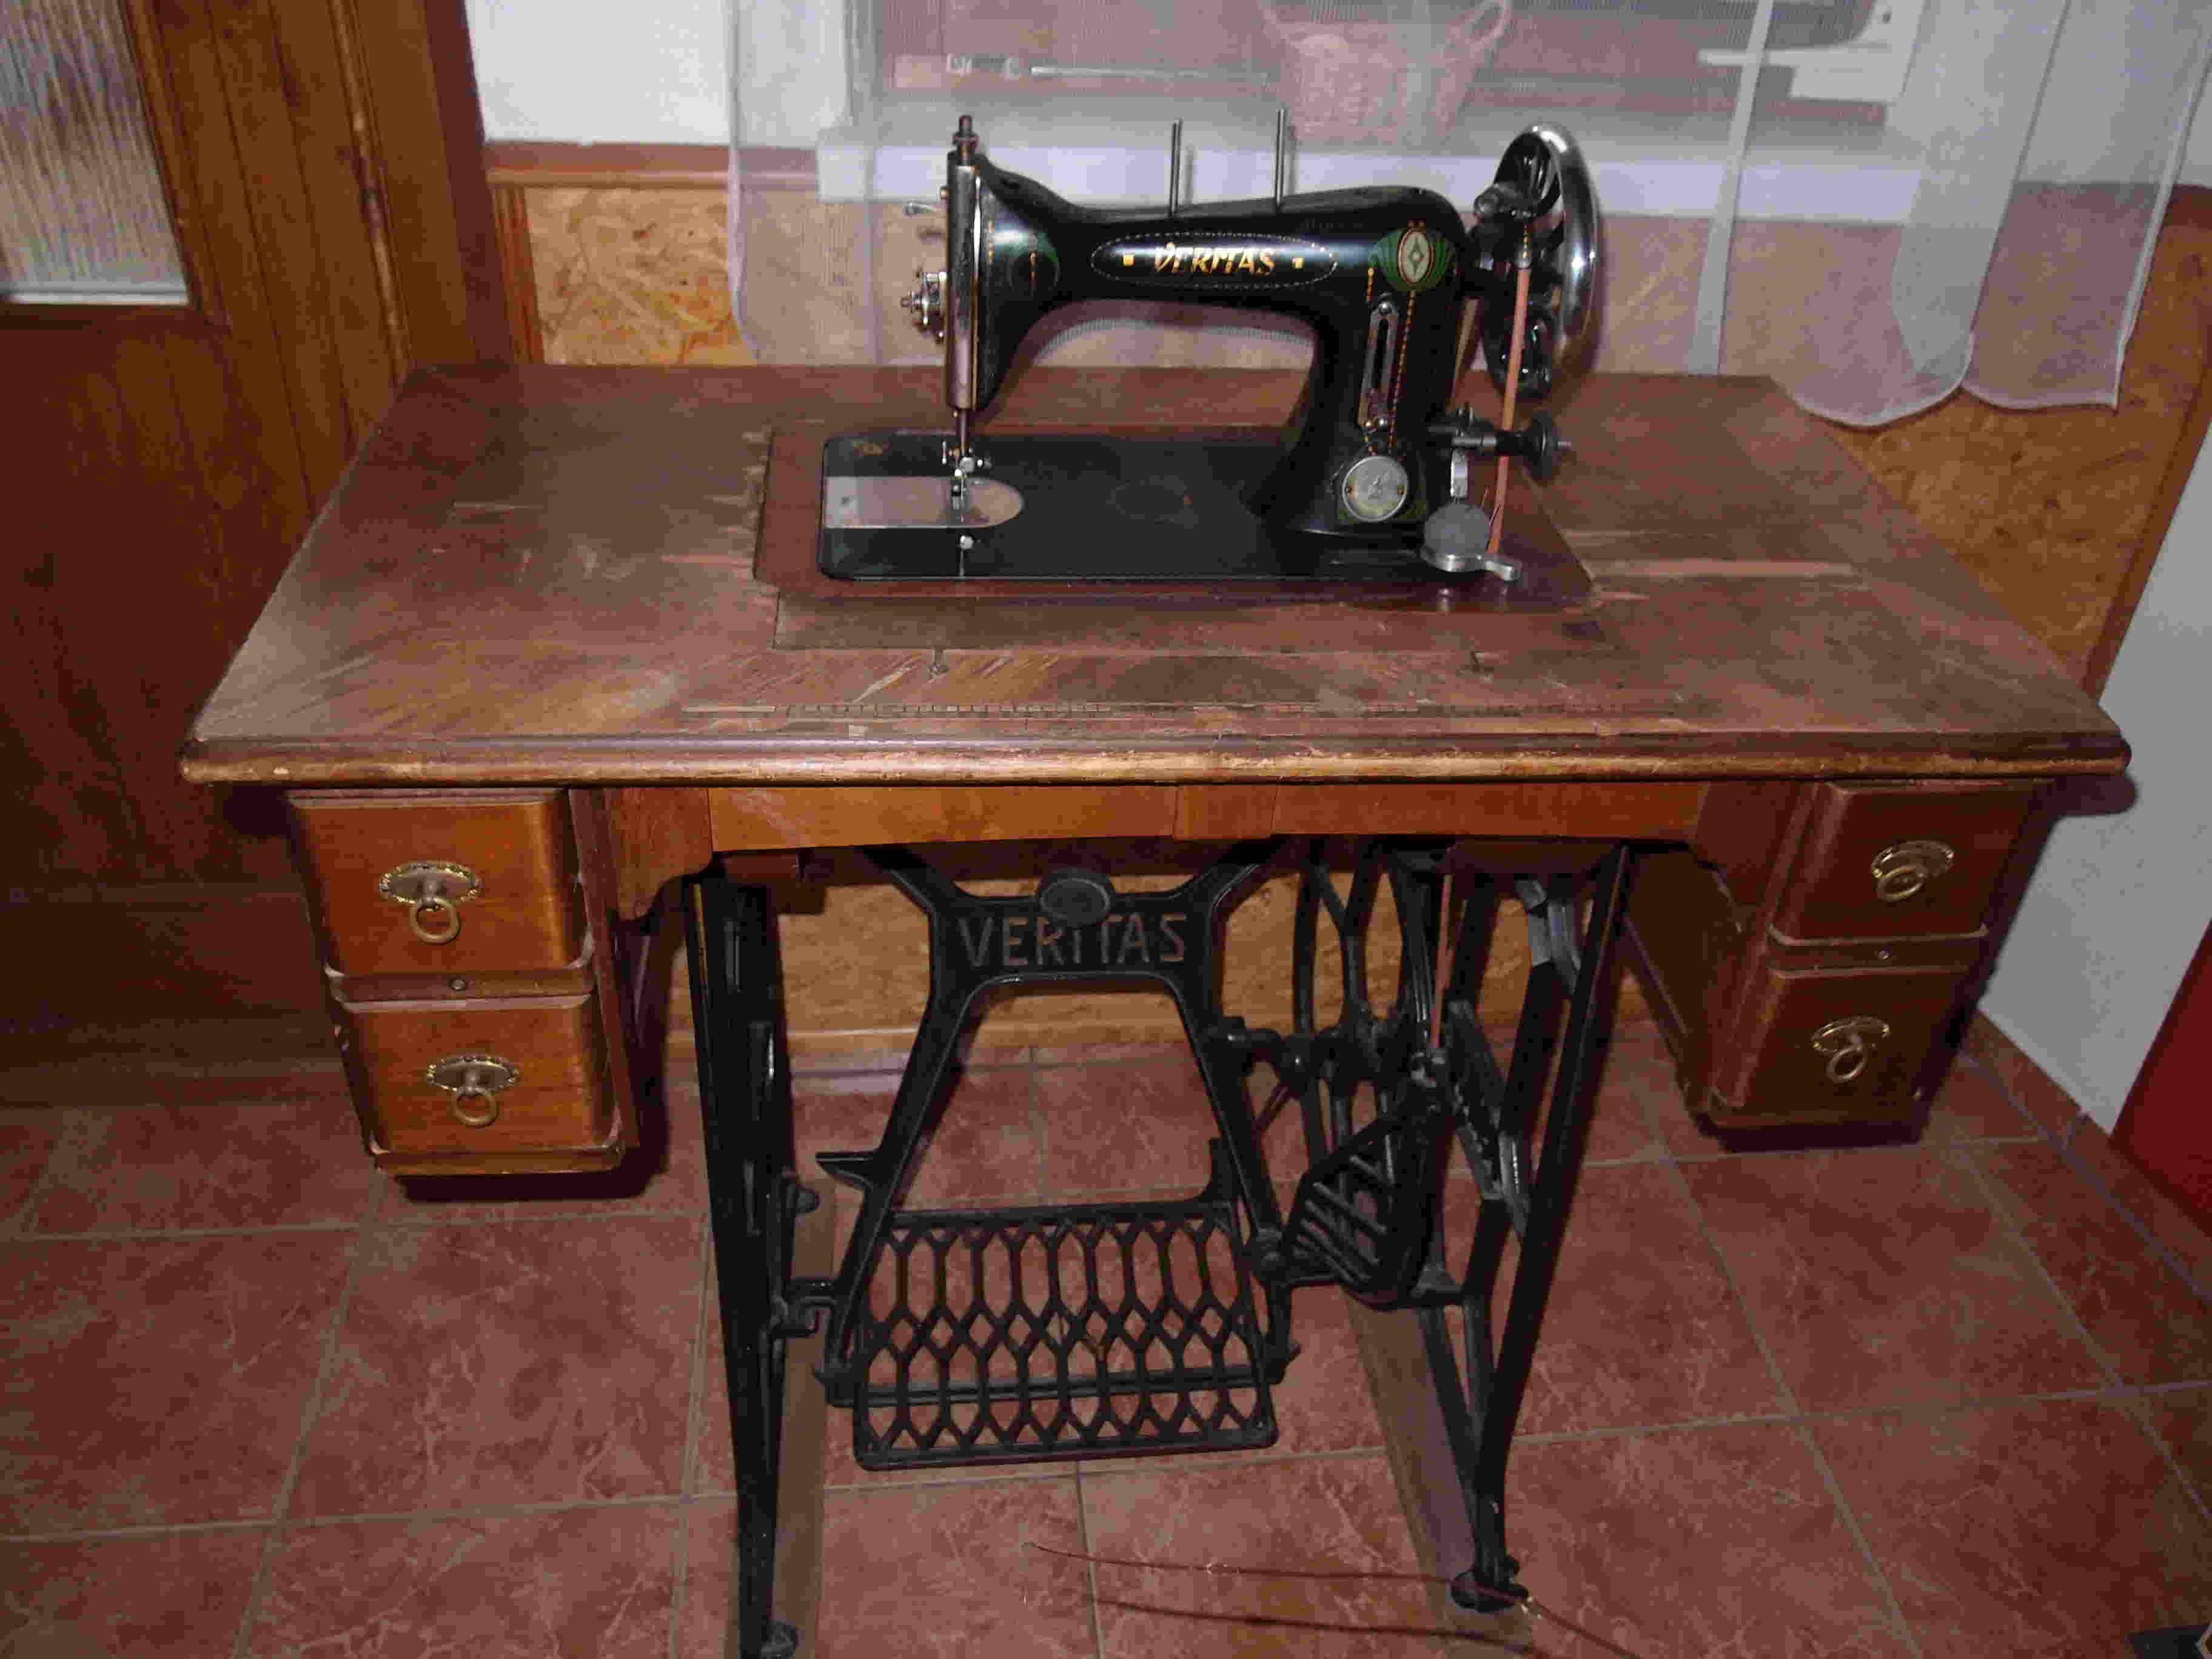
\includegraphics[scale=0.3]{img/stroj_mech.jpg}};
		\end{tikzpicture}
    \end{center}
\end{frame}

\begin{frame}
    \frametitle{Vývoj techniky -- elektromotor}
    \begin{center}
        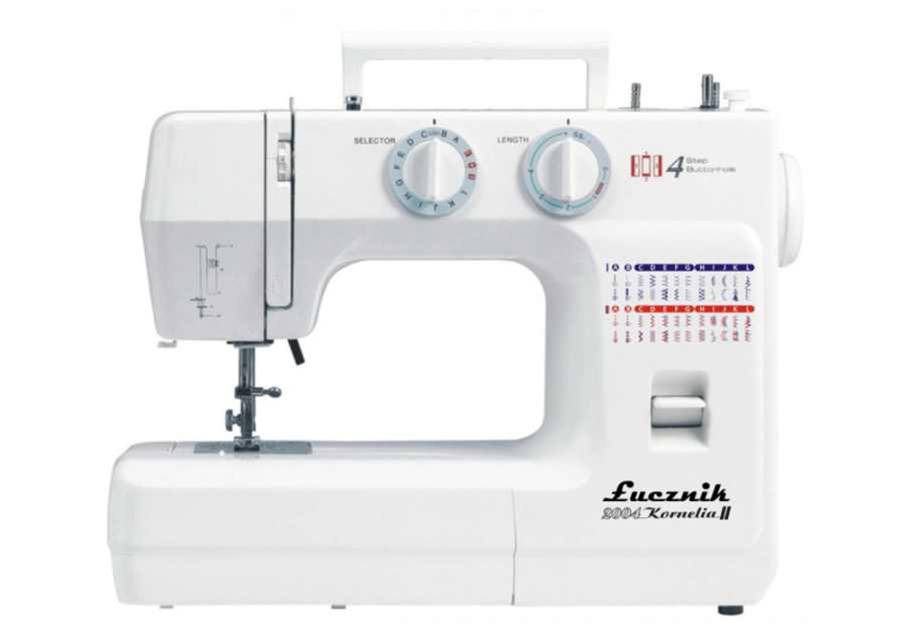
\includegraphics[scale=0.45]{img/stroj_motor.jpg}
    \end{center}
\end{frame}

\begin{frame}
    \frametitle{Vývoj techniky -- elektronika}
    \begin{center}
		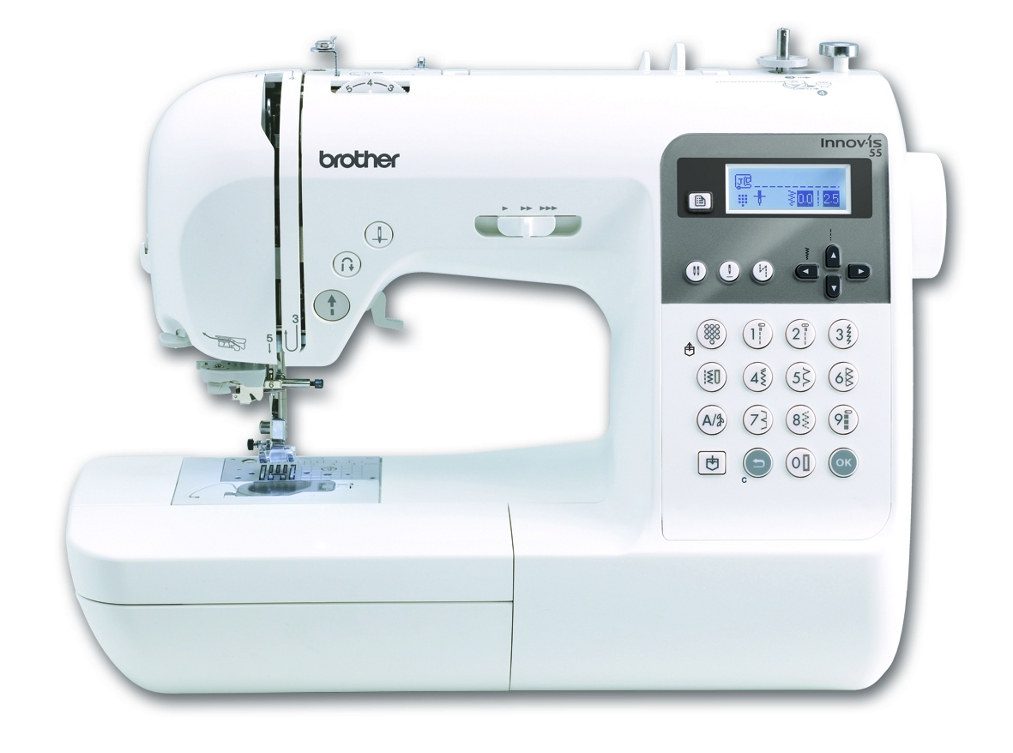
\includegraphics[scale=0.26]{img/stroj_ele.jpg}
    \end{center}
\end{frame}


\begin{frame}
	\frametitle{Vývoj směřuje k elektronice a mikročipům}
	\begin{columns}
		\column{.5\textwidth}
   			\begin{center}
		    \begin{tikzpicture}
\node[drop shadow={shadow xshift=.8ex,shadow yshift=-.8ex},fill=white,draw] at (0,0) {   		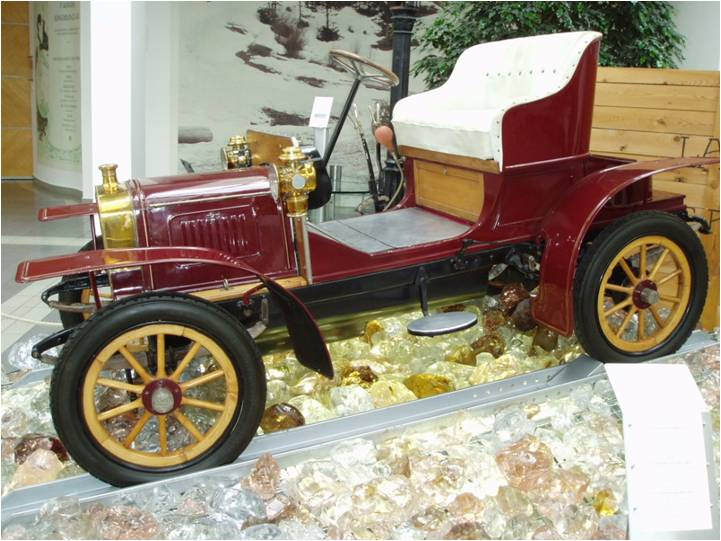
\includegraphics[scale=0.4]{img/car_old.jpg}};
			\end{tikzpicture}
			\end{center}
		\column{.5\textwidth}
			\begin{center}
		    \begin{tikzpicture}
\node[drop shadow={shadow xshift=.8ex,shadow yshift=-.8ex},fill=white,draw] at (0,0) {   		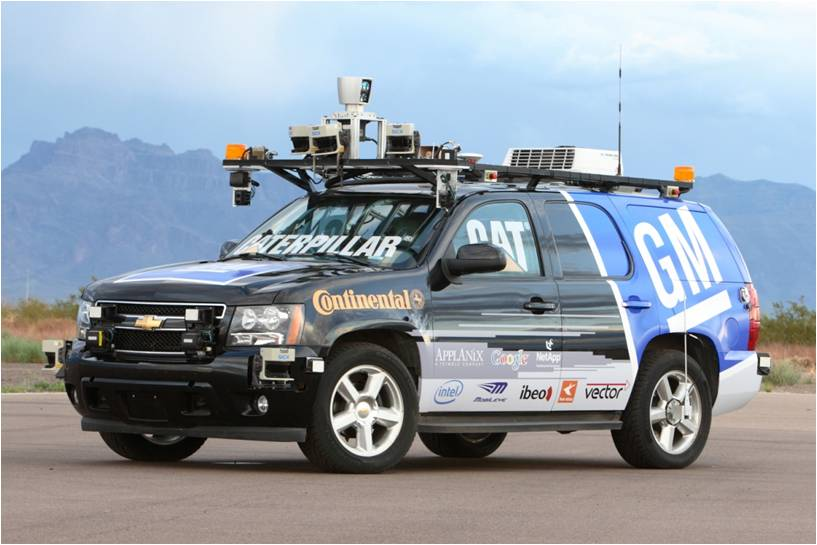
\includegraphics[scale=0.4]{img/car_new.jpg}};
			\end{tikzpicture}
			\end{center}
	\end{columns}
\end{frame}


\begin{frame}
    \frametitle{Vývoj směřuje k elektronice a mikročipům}
    \begin{center}
		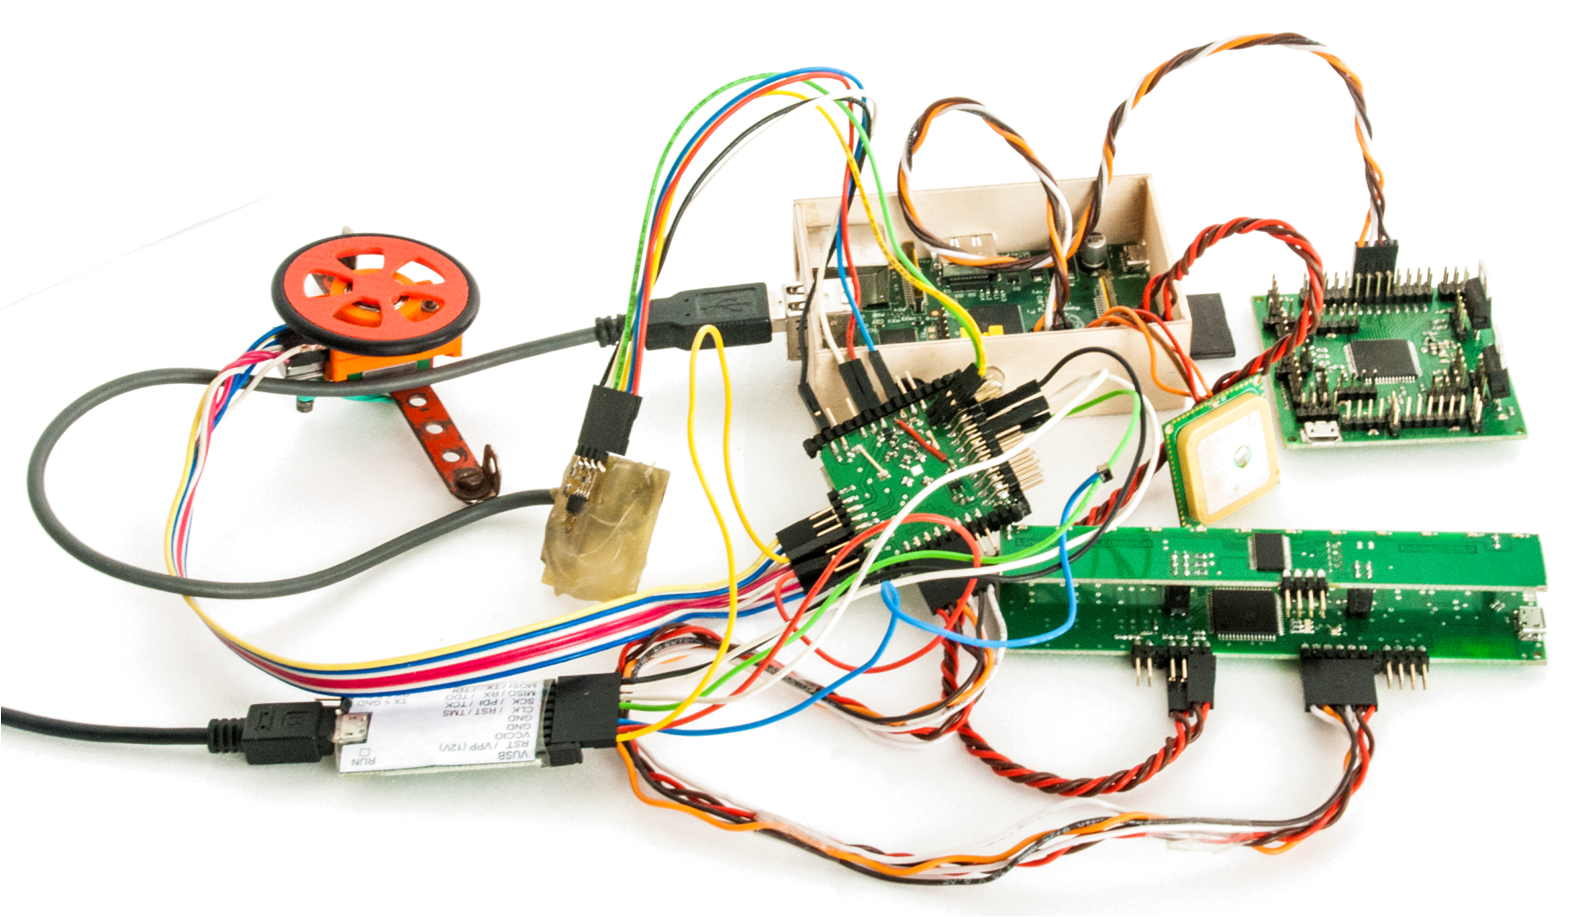
\includegraphics[scale=0.45]{img/pavouk.png}
    \end{center}
\end{frame}



\begin{frame}
	\frametitle{Nástroje pro vývojáře -- mechanika}
	\begin{columns}
		\column{.4\textwidth}
   			\begin{center}
		    \begin{tikzpicture}
\node[drop shadow={shadow xshift=.8ex,shadow yshift=-.8ex},fill=white,draw] at (0,0) {   		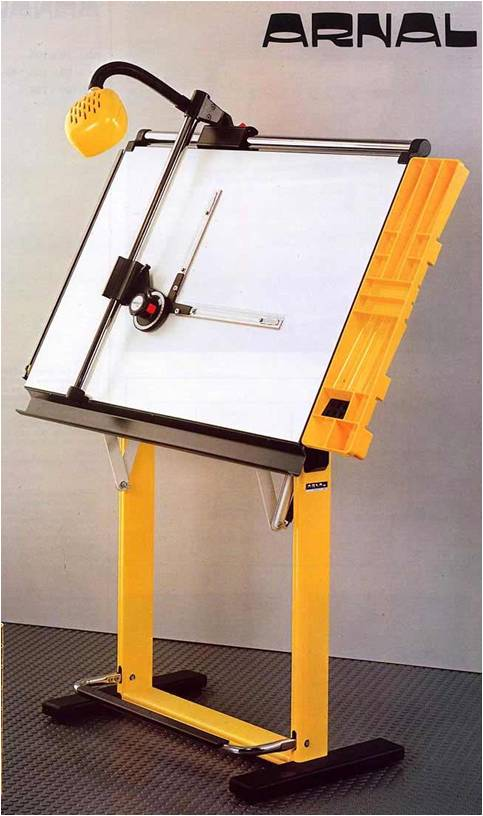
\includegraphics[scale=0.4]{img/eng_old.jpg}};
			\end{tikzpicture}
			\end{center}
		\column{.6\textwidth}
			\begin{center}
		    \begin{tikzpicture}
\node[drop shadow={shadow xshift=.8ex,shadow yshift=-.8ex},fill=white,draw] at (0,0) {   		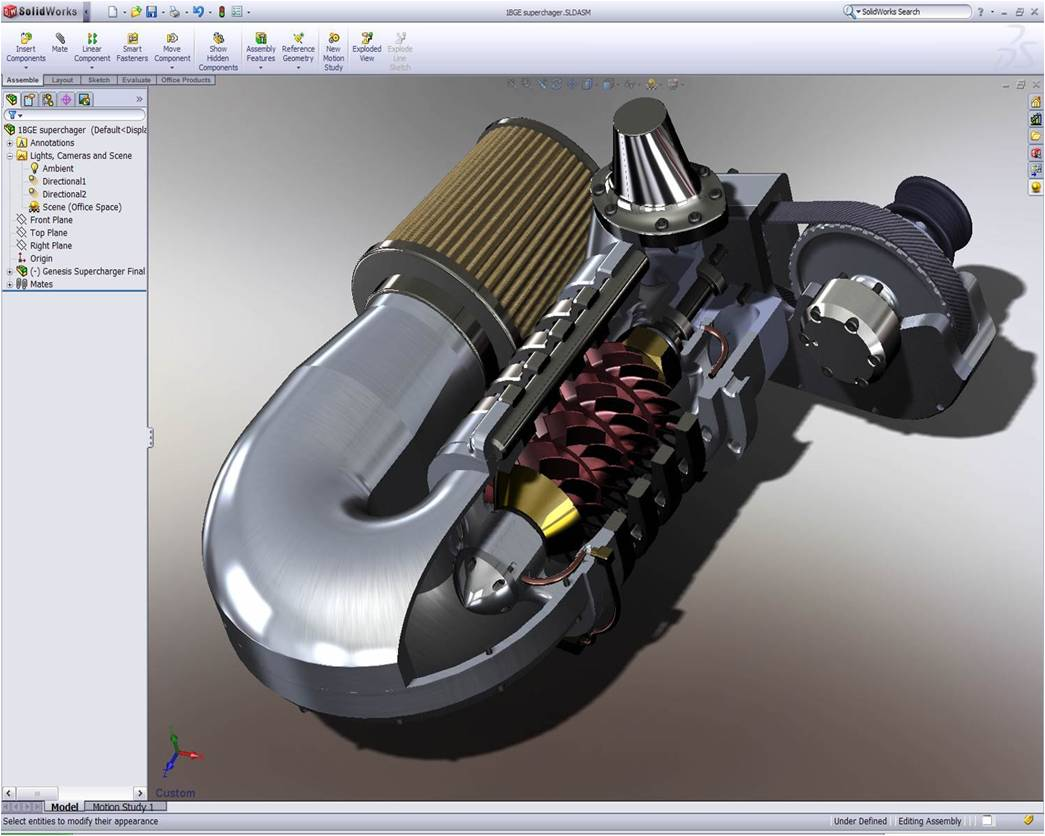
\includegraphics[scale=0.37]{img/eng_new.jpg}};
			\end{tikzpicture}
			\end{center}
	\end{columns}
\end{frame}

\begin{frame}
	\frametitle{Nástroje pro vývojáře -- elektronika}
	\begin{columns}
		\column{.5\textwidth}
   			\begin{center}
		    \begin{tikzpicture}
\node[drop shadow={shadow xshift=.8ex,shadow yshift=-.8ex},fill=white,draw] at (0,0) {   		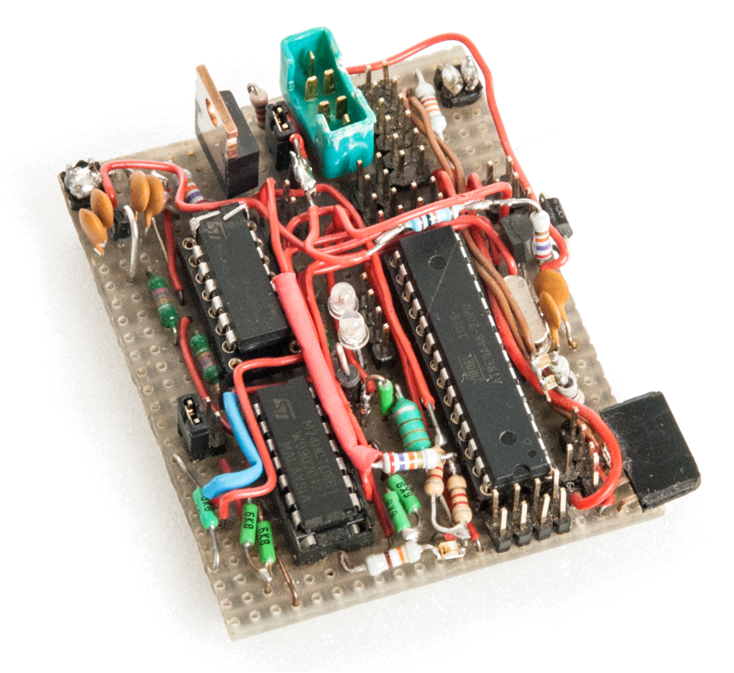
\includegraphics[scale=0.4]{img/ele_old.png}};
			\end{tikzpicture}
			\end{center}
		\column{.5\textwidth}
			\begin{center}
		    \begin{tikzpicture}
\node[drop shadow={shadow xshift=.8ex,shadow yshift=-.8ex},fill=white,draw] at (0,0) {   		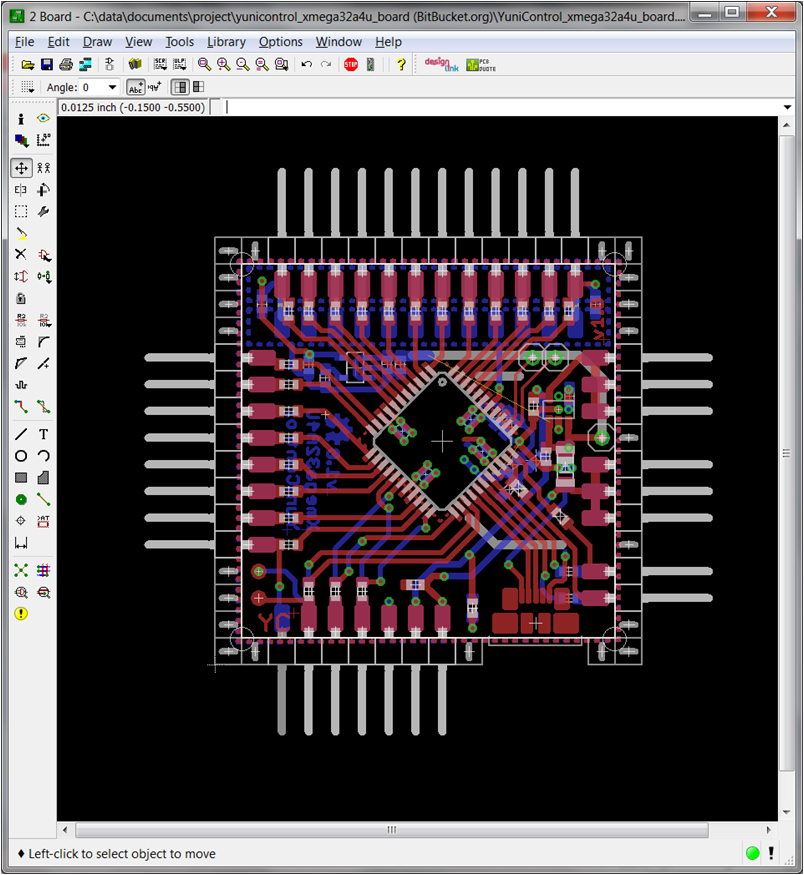
\includegraphics[scale=0.4]{img/ele_new.png}};
			\end{tikzpicture}
			\end{center}
	\end{columns}
\end{frame}


\begin{frame}
    \frametitle{Nástroje pro vývojáře -- programátor mikročipů}
    \begin{center}
	    \begin{tikzpicture}
		  \node[drop shadow={shadow xshift=.8ex,shadow yshift=-.8ex},fill=white,draw] at (0,0) {   		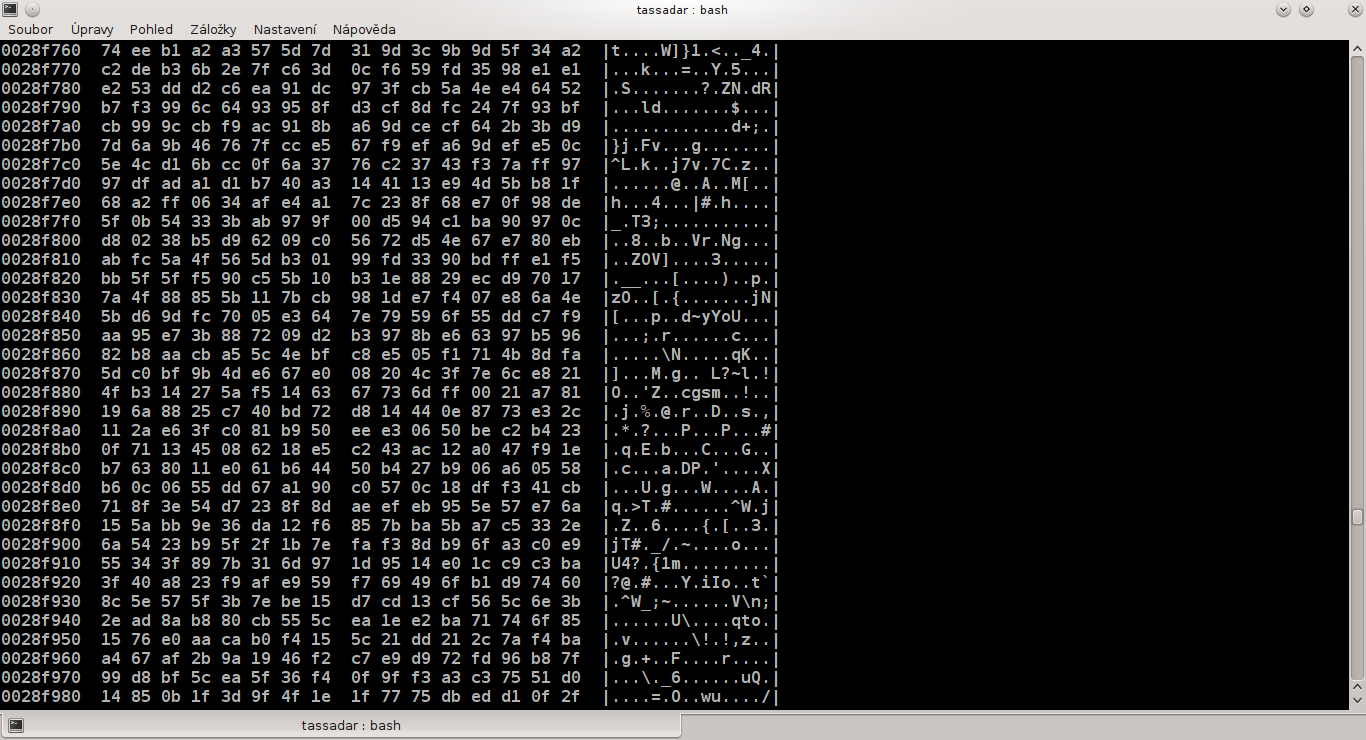
\includegraphics[scale=0.33]{img/prog.png}};
		\end{tikzpicture}
    \end{center}
\end{frame}


\begin{frame}
    \frametitle{Požadavky}		
    \begin{columns}
		\column{.5\textwidth}
			\begin{center}
			\begin{enumerate}
				\item Přehledné zobrazení proudu dat
				\item Podpora rozličných formátů
				\item Intuitivní používání
			\end{enumerate}
			\end{center}
		\column{.5\textwidth}
			\begin{center}
			\begin{enumerate}
				\setcounter{enumi}{3}
				\item Snadná rozšiřitelnost
				\item Nezávislost na další aplikaci
				\item Nízká cena
			\end{enumerate}
			\end{center}
	\end{columns}	
	
	\begin{center}
    \begin{tabular}{ | l | l | l | l | l | l | l | l |}
        \hline                     %                            oss      nezavislost cena 
        Požadavky:                  & 1      & 2      & 3       & 4      & 5      & 6      & cena      \\ \hline
        LabVIEW                     & \Has   & \Has   & \NoHas  & \NoHas & \Has   & \NoHas & 65000,- kč\\ \hline
        MATLAB+Simulink             & \Has   & \Has   & \NoHas  & \NoHas & \Has   & \NoHas & 95000,- kč \\ \hline
        ControlWeb                  & \Has   & \Has   & \NoHas  & \NoHas & \Has   & \NoHas & 19000,- kč \\ \hline
    %    SerialChart                 & \Has   & \NoHas & \Has    & \Has   & \Has   & \Has   & Open-source \\ \hline 
        WinWedge                    & \NoHas & \Has   & \Has    & \NoHas & \NoHas & \NoHas & 5000,- kč \\ \hline 
        Advanced Serial Data Logger & \NoHas & \Has   & \Has    & \NoHas & \NoHas & \NoHas & 2000,- kč \\ \hline 
        StampPlot Pro               & \Has   & \Has   & \NoHas  & \NoHas & \Has   & \Has   & Freeware  \\ \hline 
    %    Lorris                      & \Has   & \Has   & \Has    & \Has   & \Has   & \Has  \\ \hline 
    \end{tabular}
    \end{center}
\end{frame}


\begin{frame}
    \frametitle{Lorris~~~~~~~~~~~~~~~~~~~~~~~~~~~~~~~~~~~~~~~~~~~~~~~~~~~~~~~~~~~~~~~~~~~~~~.}
    \begin{center}
	    \begin{tikzpicture}
		  \node[drop shadow={shadow xshift=.8ex,shadow yshift=-.8ex},fill=white,draw] at (0,0) {   		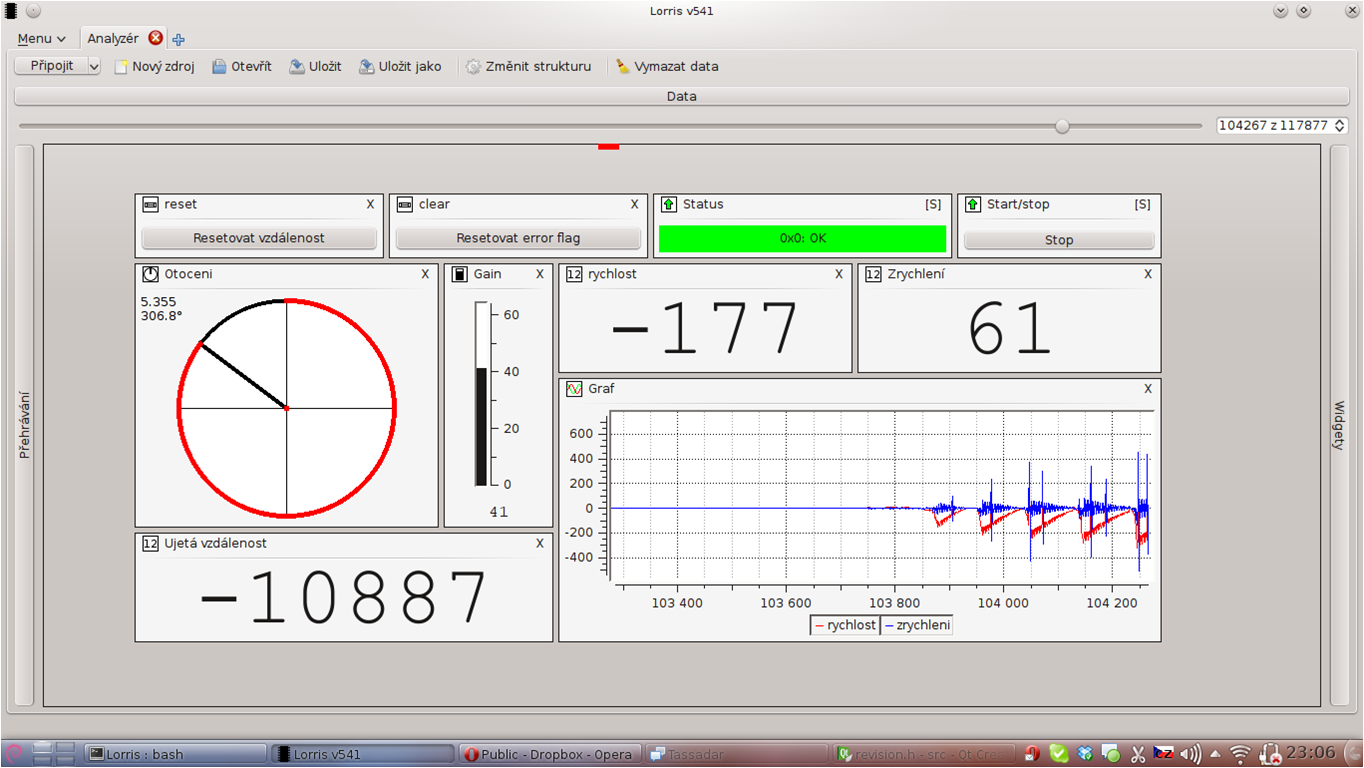
\includegraphics[scale=0.43]{img/analyzer.png}};
		\end{tikzpicture}
    \end{center}
\end{frame}

\begin{frame}
\frametitle{Přínos}		
    \begin{columns}
	\column{.48\textwidth}
		\begin{negativeblock}{bez Lorris}
		\begin{itemize}
			\item Data pouze v terminálu
			\item Nastavování vždy znovu
			\item Složité hledání chyb
			\item Mnoho nástrojů
		\end{itemize}
		\end{negativeblock}
	\column{.48\textwidth}
		\begin{positiveblock}{s Lorris}
		\begin{itemize}
			\item Grafické zobrazení dat
			\item Ukládání do sezení
			\item Jednodušší hledání chyb
			\item Vše na jednom místě
		\end{itemize}
		\end{positiveblock}
	\end{columns}
\end{frame}

\begin{frame}
    \frametitle{Lorris mobile}
    \begin{center}
		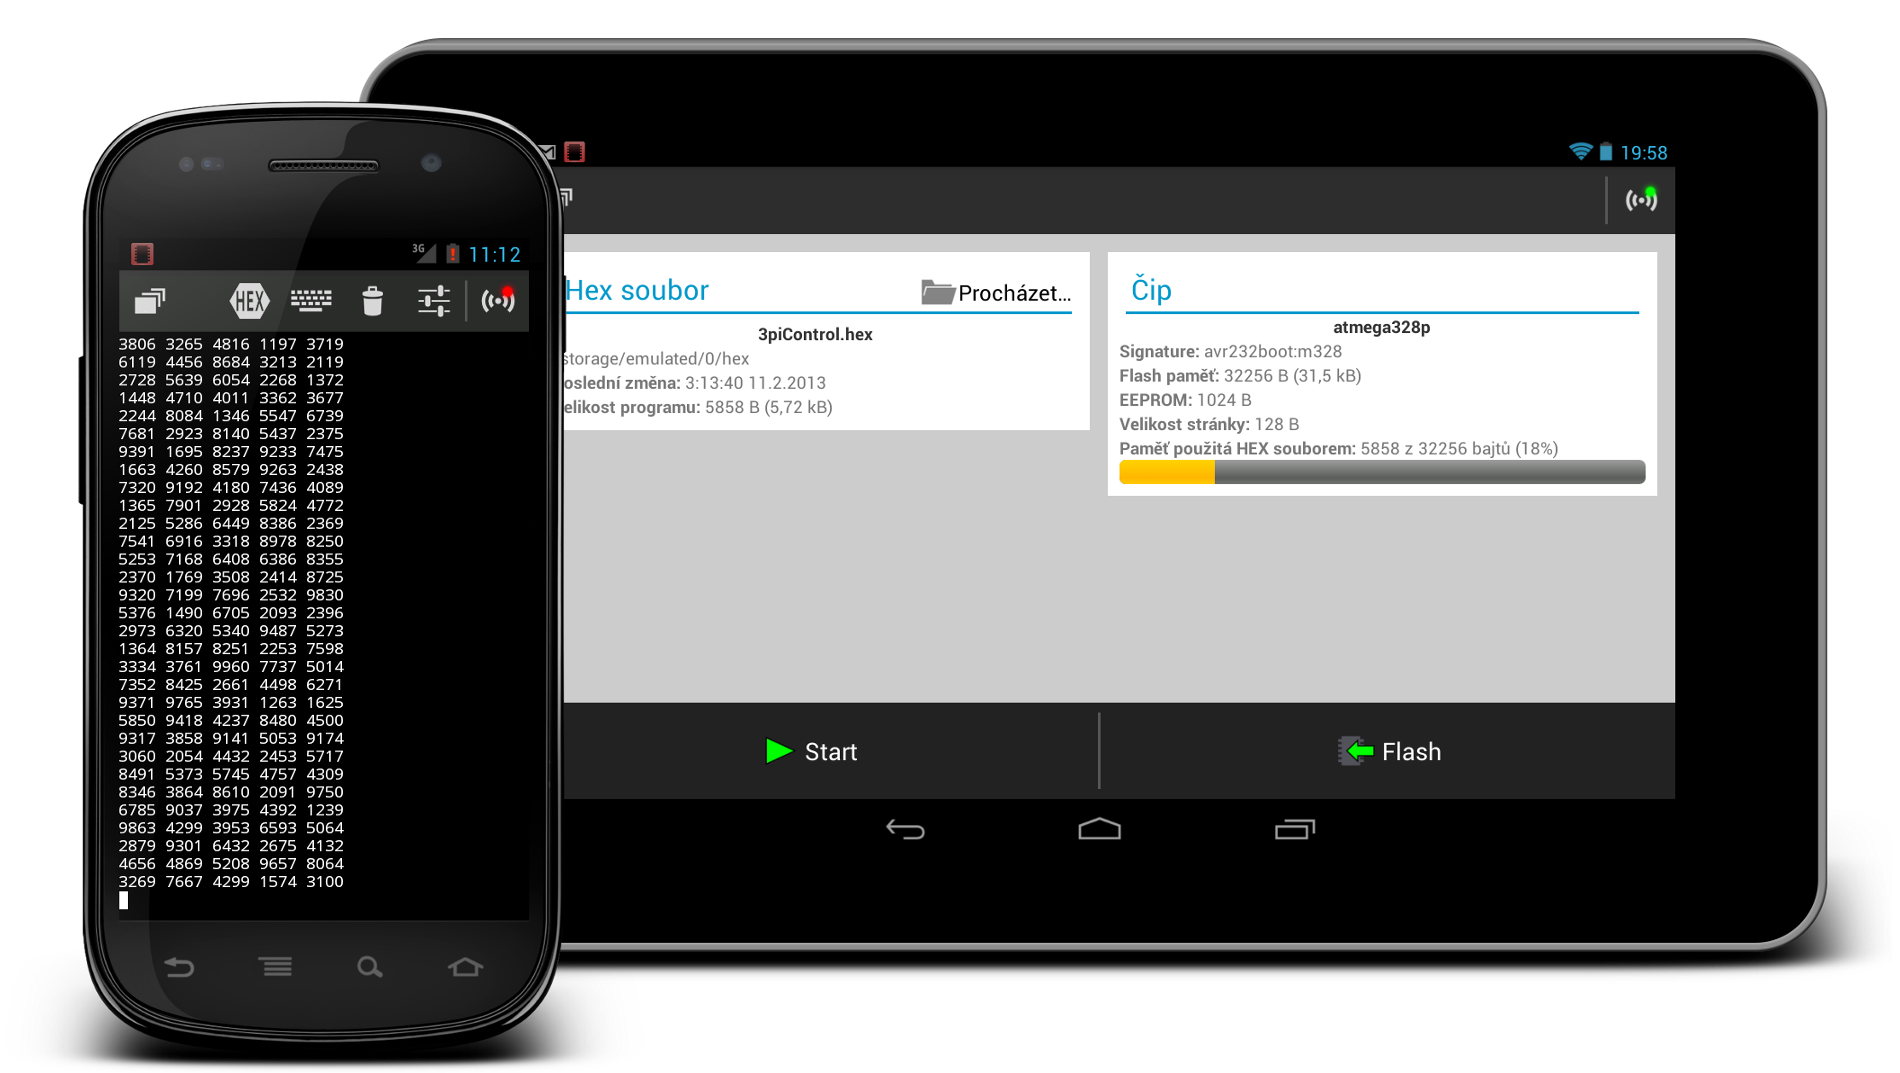
\includegraphics[width=\textwidth]{img/mobile_programmer.png}
    \end{center}
\end{frame}


\begin{frame}	
	\begin{center}
		{\huge Děkuji za pozornost}
		\vspace{20mm}
		\\
		\url{http://tasssadar.github.io/Lorris}
		\url{http://tasssadar.github.io/Lorris/cz}
	\end{center}
\end{frame}

\end{document}